\section{Trajectory analysis} \label{ch:trajectory}

**intro**

\subsection{Governing equations}\label{sec:gov}

\begin{wrapfigure}{r}{0.4\textwidth}
		\centering
		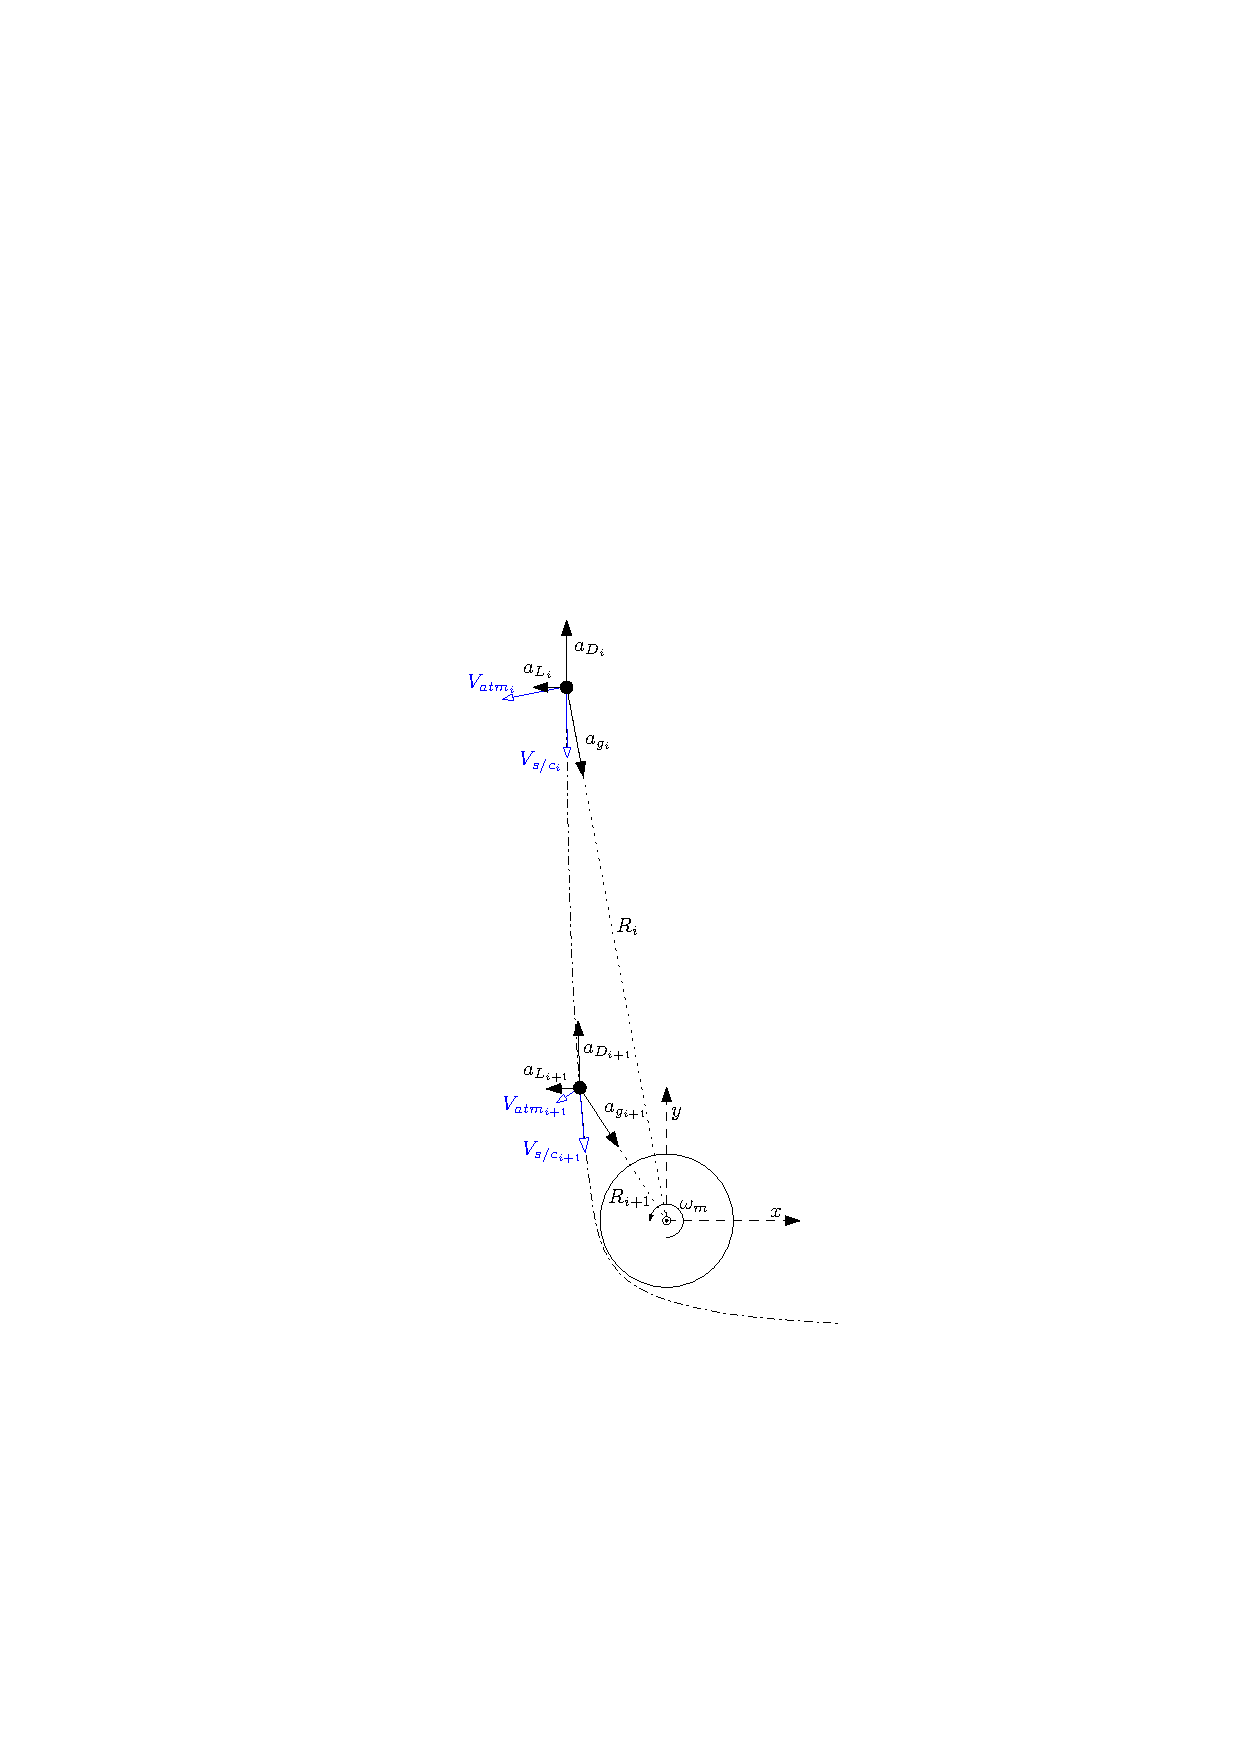
\includegraphics[width = 0.4\textwidth]{Figure/orbital_mechanics.pdf}
		\caption{The kinetic diagram visualizing the governing equations of the trajectory analysis}
		\label{fig:orb}
\end{wrapfigure}

The motion of a spacecraft can be broken down in some dominant contributors. These contributors are the gravitational pull and the aerodynamic forces. Disturbances like solar radiation or gravitational pull from moons or other bodies is neglected in the model.

To be able to fully describe the contributors, two reference frames need to be defined. The non rotating inertial frame is defined with its origin in the centre of mass of Mars if it would be perfectly spherical, this is the \gls{mci}. 
Another reference frame is the \gls{mcmf}. in our first model the origin and the z-axis of both reference frames is equal (so no axis tilt is taken into account). The difference between the two is that the \gls{mcmf} is rotating around the z-axis with rotational velocity \gls{con:omegamars} compared to the \gls{mci}.

The gravitational pull is described by Newtons law of gravitation, together with Newton's second law, it can be written as an acceleration as in equation \ref{eq:nG}.

\begin{equation} \label{eq:nG}
\gls{sym:g} = -\frac{\gls{con:G}\gls{con:Mmars}}
					{\gls{sym:R}^3}\gls{sym:Rv}
\end{equation}

The aerodynamic forces are described by the lift and the drag, these forces are acting in the direction and orthogonal to the velocity of the spacecraft with respect to the atmosphere, this is the velocity of the spacecraft in the \gls{mcmf}. To make be able to express the aerodynamic forces in the \gls{mci} this velocity needs to be converted to \gls{mci} as in equation \ref{eq:Vsc_mcmf_mci}.

\begin{equation} \label{eq:Vsc_mcmf_mci}
\left.\gls{sym:Vvsc}\right|_{MCMF}^{MCI} = \gls{sym:Vvsc}_{,a} = \left.\gls{sym:Vvsc}\right|_{MCI} - \left(\gls{con:Omegamars} \times \gls{sym:Rv} \right)
\end{equation}

The aerodynamic accelerations due to the lift and the drag are described by equations \ref{eq:aL} and \ref{eq:aD} respectively.

\begin{equation} \label{eq:aL}
\gls{sym:aL} = \frac{\gls{sym:CL}\gls{sym:rho}\gls{sym:A}}{2 \gls{sym:m}} 
				\left|\gls{sym:Vvsc}_{,a}\right|^2
				\frac{\gls{sym:Vvsc}_{,a} \times \mathbf{z}}
				{\left| \gls{sym:Vvsc}_{,a} \times \mathbf{z}\right|}
\end{equation}

\begin{equation} \label{eq:aD}
\gls{sym:aD} = \frac{\gls{sym:CD}\gls{sym:rho}\gls{sym:A}}{2 \gls{sym:m}}
				\left|\gls{sym:Vvsc}_{,a}\right|^2 \frac{\gls{sym:Vvsc}_{,a}}{\left|\gls{sym:Vvsc}_{,a}\right|}
\end{equation}

\subsection{Program structure}\label{sec:prog_struct}

In order to use the equations of motion to produce usefull results

**Modules
****Orbit
****Full orbit
****orbit selection
**flowchart
\begin{figure}[H]
%\centering
\hspace{-23mm}
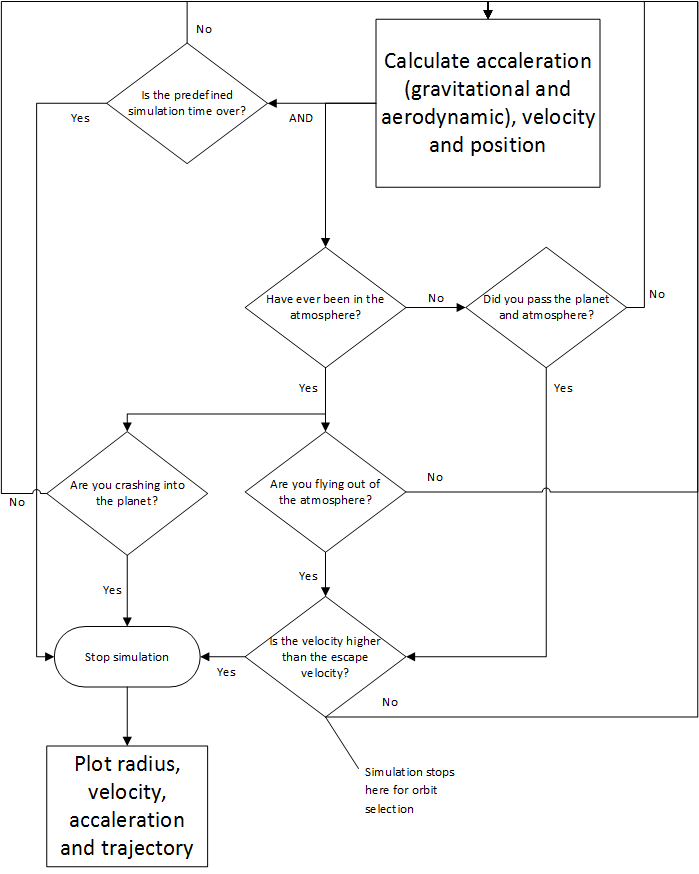
\includegraphics[width = 0.8\textwidth]{Figure/astro_tool.png}
\vspace{-5mm}
\caption{Flowchart of the working principle of the trajectory analysis program}
\label{fig:traj_flow}
\end{figure}

\subsection{Verification and validation}